\documentclass{paper}
\usepackage[UTF8]{ctex}
\usepackage{graphicx}  %插入图片
\usepackage[export]{adjustbox}
\usepackage{float}
\usepackage{geometry}
\usepackage{amssymb}
\usepackage{indentfirst}
% \usepackage{biblatex}
\usepackage[ruled,linesnumbered]{algorithm2e}
\usepackage[colorlinks,linkcolor=blue,bookmarksopen=true,bookmarksnumbered=true]{hyperref}
\usepackage{pythonhighlight}
\usepackage{color}

\setlength{\parindent}{4em}
\setlength{\parskip}{1em}
\geometry{a4paper,scale=0.8}
\SetKwInput{KwIn}{输入}
\SetKwInput{KwOut}{输出}

\begin{document}

% 目录
\tableofcontents
\newpage

\section{实验要求}
	\begin{itemize}
		\item 实现决策树桩(Decision Tree Stump)算法。
		\item 实现逻辑回归(Logistic Regression)算法。
		\item 基于上述两个分类器实现自适应增强(Adaptive Boost,Adaboost)算法,使得该算法可以选择基分类器(Base Classifier)的类型以及基分类器的数目。
		\item 实现上述算法时不使用任何机器学习模型库。

                在本实验中,仅模型使用numpy完成。

		\item 将给定的数据集(Data Set)随机划分成10个子集,使用其中一个子集作为验证集(Validation Set),并使用Adaboost算法对模型进行训练和交叉验证。
		\item 将实现的Adaboost算法封装成Python脚本,并使用命令行参数暴露接口,使得算法可以指定基分类器的类别,新的测试数据的目录以及输出文件的目录。
	\end{itemize}



\section{算法设计与实现}
	\subsection{Adaboost算法}

	    Adaboost算法是一种集成学习方法,它通过组合多个弱分类器来构建一个强分类器。在每次迭代中,Adaboost算法会根据上一次迭代的结果调整样本权重,使得上一次分类错误的样本权重变大,而分类正确的样本权重变小。这样,Adaboost算法能够更加关注那些难以分类的样本,从而提高分类的准确率。

	    Adaboost算法的基本思想是将多个弱分类器组合成一个强分类器。在每次迭代中,Adaboost算法会根据上一次迭代的结果调整样本权重,使得上一次分类错误的样本权重变大,而分类正确的样本权重变小。这样,Adaboost算法能够更加关注那些难以分类的样本,从而提高分类的准确率。

\subsubsection{Adaboost算法实现}
	
首先初始化一个向量$\mathcal{D}_1 = [\frac{1}{m}]_{1 \times m}$作为最初的样本权重。接着进行$\mathcal{T}$轮迭代。在每一轮迭代中以样本权重$\mathcal{D}_i$计算加权训练分类器$h_i$并计算加权错误率$\epsilon$,接着使用公式$\alpha_{i} \leftarrow {1 \over 2} \ln {1-\epsilon \over \epsilon}$计算,接着使用公式$\mathcal{D}_{i+1} \leftarrow \mathcal{D}_i \odot \exp(-\alpha_i \mathbb{I}(h_i(\mathbf{x}) = y))$计算新的样本权重,最后对权重进行归一化。迭代结束后算法返回$sign(\sum_{t \epsilon [\mathcal{T}]}{\alpha}_t h_t)$作为最终的分类器。

	    详细的Adaboost算法介绍参考文献:\cite{ref1}。

	    % 伪代码见算法1 $\leftarrow$ 这里要能够转调到算法部分
	    伪代码见算法\ref{alg:1}。

	    \newpage

		\begin{algorithm}[H]
			\label{alg:1}
			\SetAlgoLined
			\caption{Adaboost算法}
			
			\KwIn{训练数据集$\mathcal{S}=\{(\mathbf{x_i},y_i)\}_{i\epsilon[m]}$,基分类器算法$\mathcal{L}$,基分类器数目(迭代次数)$\mathcal{T}$}
			
			$\mathcal{D}_1 \leftarrow [{1 \over m}]_{1 \times m}$  \tcp*[R]{初始化权重}
			
			\For{$t \leftarrow 1$ \KwTo $\mathcal{T}$}
			{
                $h_t \leftarrow \mathcal{L}(\mathcal{S},\mathcal{D}_t)$  \tcp*[R]{以样本权重$\mathcal{D}_t$训练$h_t$} \label{algpart:1}

				$\epsilon \leftarrow \mathcal{D}_t \odot \mathbb{I}(h_t(\mathbf{x}) \neq y)$ \tcp*[R]{计算训练集的加权错误率} \label{algpart:2}

				\lIf{$\epsilon \textgreater 0.5$}{break} \label{algpart:4}

				$\alpha_{t} \leftarrow {1 \over 2} \ln {1-\epsilon \over \epsilon}$

				$\mathcal{D}_{t+1} \leftarrow \mathcal{D}_t \odot \exp(-\alpha \mathbb{I}(h_t(\mathbf{x}) = y))$

				$s \leftarrow \sum \mathcal{D}_t$

				$\mathcal{D}_t \leftarrow {\mathcal{D}_t \over s}$ \tcp*[R]{权重归一化}
			}


			\KwOut{$sign(\sum_{t \epsilon [\mathcal{T}]}{\alpha}_t h_t)$}
            \label{algpart:3}
	  \end{algorithm}

算法具体实现下图:
\begin{figure}[H]
    \centering
    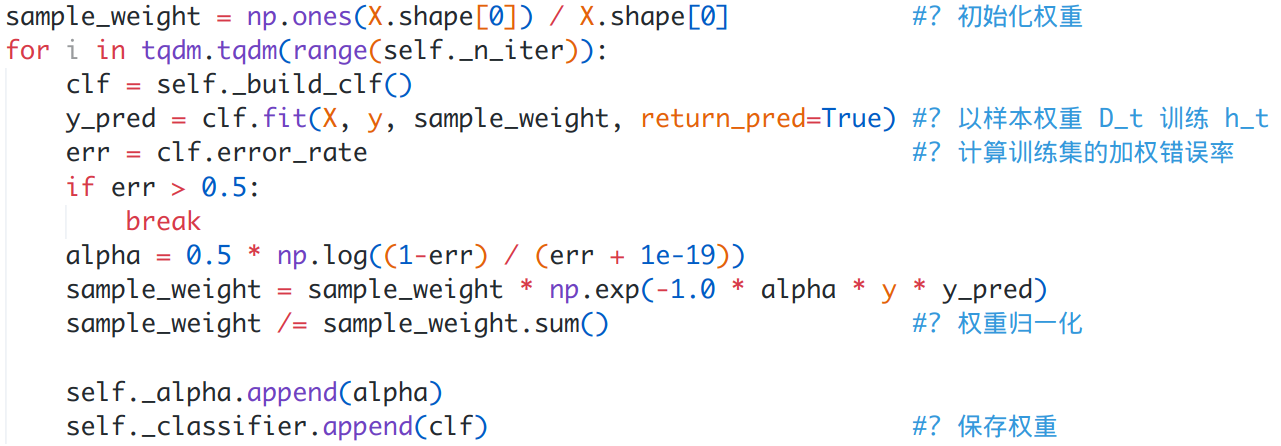
\includegraphics[scale=0.35, frame]{images/adaboost.png}
    \caption{Adaboost算法实现}
\end{figure}

\subsection{分类器需要暴露的接口}

\begin{enumerate}
    \item 用于训练的接口$fit(\mathcal{S},\mathcal{D}_t)$
            
            $fit$接口用于实现算法伪代码中的步骤\ref{algpart:1}:实现以样本权重$\mathcal{D}_t$训练$h_t$。

            $DecisionTreeStump$的$fit$接口实现见: \ref{d:f}。

            $LogisticRegression$的$fit$接口实现见: \ref{l:f}。
    
    \item 用于预测的接口$predict(\mathbf{x})$
    
            $predict$接口用于实现算法伪代码中的步骤\ref{algpart:2}:计算训练集的加权错误率。

            $DecisionTreeStump$的$predict$接口实现见: \ref{d:p}。

            $LogisticRegression$的$predict$接口实现见: \ref{l:p}。
    
    \item 用于获取训练集加权错误率的接口$@property:error\_rate$
    
            $error\_rate$接口用于实现算法伪代码中的步骤\ref{algpart:2}:计算训练集的加权错误率。

    \item 用于获取分类器权重的接口$@property:weight$
            
            $weight$接口用于实现算法伪代码中的输出部分\ref{algpart:3},作为Adaboost算法模型的权重输出。
\end{enumerate}

\subsection{DecisionTreeStump实现}

$DecisionTreeStump$算法,也称单层决策树,是一种简单的决策树。它仅仅是基于单个特征来做决策。由于这棵树只有一次分裂过程,因此它实际上仅仅是一个树桩。

决策树桩详细内容见参考文献:\cite{ref2}。

\subsubsection{初始化权重以及错误率}

$DecisionTreeStump$模型的权重由以下几个部分组成:

\begin{itemize}
    \item $critical\_dimension \in \{0 \dots dimension(x_i)-1\}$
    
            在决策树算法中,我们会依次选择训练集集的一个特征维度作为进一步划分的依据。由于$DecisionTreeStump$是单层的决策树,因此仅会进行一次划分,这单次划分依据的特征维度就是$critical\_dimension$。
    
    \item $thredhold \in \mathbb{R}$

            $thredhold$即阈值,作为所选择的特征的分界线。确定训练集的$critical\_dimension$后,使用该特征作为划分正负类样本的依据。根据样本$critical\_dimension$的值是否小于$thredhold$,将样本分成两类。

    \item $compare\_method \in \{0, 1\}$
    
            $compare\_method$即比较方法,用于划分正负类样本。
            
            \begin{itemize}
            
                \item 当$compare\_method = 0$时,$value(critical\_dimension) < thredhold$的样本将会被划分成负类;
            
                \item 当$compare\_method = 1$时,$value(critical\_dimension) \geq thredhold$的样本将会被划分成负类。
            \end{itemize}
\end{itemize}

在开始训练前,权重将会被初始化为$None$,加权错误率$err$将会被初始化为1。

\subsubsection{$DecisionTreeStump::fit(\mathcal{S},\mathcal{D})$接口实现}  \label{d:f}

对训练集的特征维度进行遍历,目的是找到最好的特征维度作为$critical\_dimension$。在每一次遍历的过程中,在特征维度的最小值和最大值之间均匀取点作为$thredhold$。接着对于$compare\_method \in \{0, 1\}$的两种取值,计算当前的加权错误率$err$。

执行完上述步骤后选取加权错误率$err$最小的特征维度、阈值以及比较方法分别作为$critical\_dimension$,$thredhold$以及$compare\_method$。

伪代码见算法\ref{alg:2}

\begin{algorithm}[H]
    \SetAlgoLined
    \label{alg:2}
    \caption{DecisionTreeStump:fit}
    \KwIn{训练数据集$\mathcal{S}=\{(\mathbf{x_i},y_i)\}_{i\epsilon[m]}$,样本权重$\mathcal{D}$}

    $steps \leftarrow 200$ \tcp*[R]{选取$thredhold$的个数}

    \For{$d \leftarrow 0 $ \KwTo $dimension(x_i)-1$}
    {
        $max \leftarrow$ 特征维度$d$上的最大值
        
        $min \leftarrow$ 特征维度$d$上的最小值

        $step\_size \leftarrow {{max - min} \over steps} $

        \For{$step \leftarrow 0$ \KwTo $steps$}
        {
            $thredhold \leftarrow min + step \cdot step\_size$ \tcp*[R]{当前遍历的阈值}

            \For{$method$ in $\{0, 1\}$}
            {
                $\hat{y} \leftarrow predict_{method,thredhold,d}(\mathbf{x})$

                $err \leftarrow <\mathbb{I}(h_t(\mathbf{x}) \neq y),\mathcal{D}>$ \tcp*[R]{计算加权误差}

                记录$err$最小的$d$、$thredhold$以及$method$ \tcp*[R]{权重保存}
            }
        }
    }

    \KwOut{$err$最小的$d$、$thredhold$以及$method$}

\end{algorithm}

具体代码见下图:
\begin{figure}[H]
    \begin{center}
        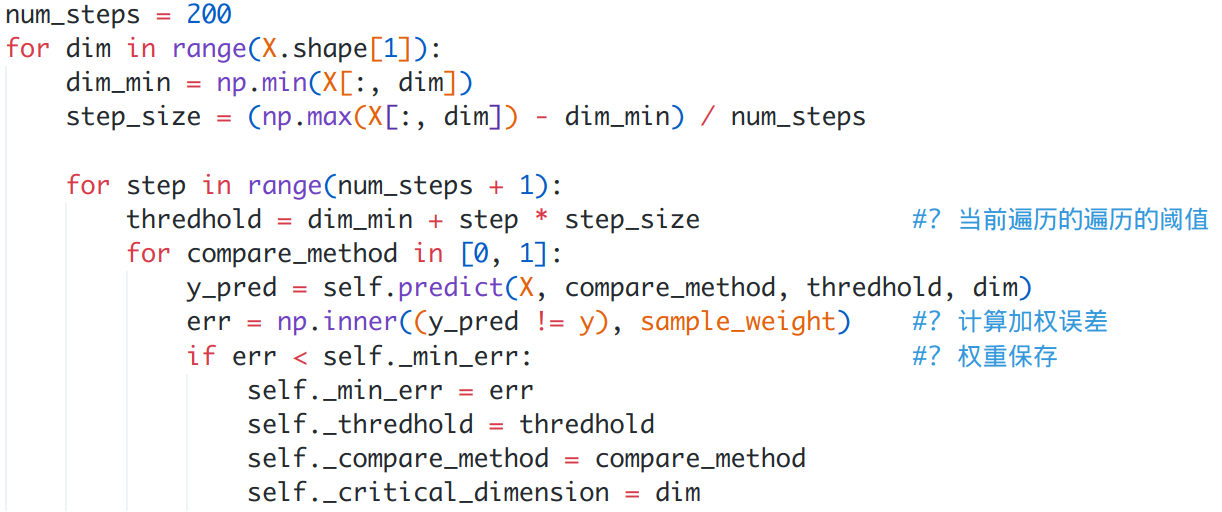
\includegraphics[scale = 0.35, frame]{images/df.png}
    \end{center}
    \caption{DecisionTreeStump::fit实现}
\end{figure}


\subsubsection{$DecisionTreeStump::predict(\mathbf{x})$接口实现} \label{d:p}

根据给定的$critical\_dimension$、$thredhold$以及$compare\_method$划分$\mathbf{x}$。

具体而言,当$compare\_method = 0$时,将$critical\_dimension$的值小于$thredhold$的样本划分成负类, 将$critical\_dimension$的值大于等于$thredhold$的样本划分成正类;当$compare\_method = 1$时,将$critical\_dimension$的值小于$thredhold$的样本划分成正类, 将$critical\_dimension$的值大于等于$thredhold$的样本划分成负类。

伪代码见算法\ref{alg:3}

\begin{algorithm}[H]
    \SetAlgoLined
    \label{alg:3}
    \caption{DecisionTreeStump:predict}
    \KwIn{数据集的特征部分$\mathbf{X}_{m \times n}$}

    $\hat\mathbf{{y}} \leftarrow [0...0]_{1 \times m}$ \tcp*[R]{$\hat{y}$作为预测值}

    \For{$i \leftarrow 0 $ \KwTo $m-1$}
    {
        $d \leftarrow critical\_dimension$

        \eIf{$\mathbf{X}_{i,d} < thredhold$}
        {
            \leIf{$compare\_method = 0$}{$\hat{y}_i \leftarrow -1$}{$\hat{y}_i \leftarrow 1$}
            
        }{
            \leIf{$compare\_method = 0$}{$\hat{y}_i \leftarrow 1$}{$\hat{y}_i \leftarrow -1$}
        }
    }

    \KwOut{$\hat{\mathbf{y}}$}
\end{algorithm}

具体代码见下图:
\begin{figure}[H]
    \begin{center}
        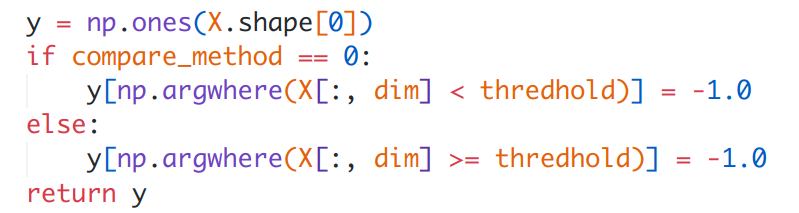
\includegraphics[scale = 0.35, frame]{images/dp.png}
    \end{center}
    \caption[short]{DecisionTreeStump::predict实现}
\end{figure}

\subsection{LogisticRegression实现}

Logistic Regression(逻辑回归)\cite{ref3}是一种用于解决二分类问题的机器学习方法,用于估计某种事物的可能性。它是一种广义线性模型,假设因变量 y 服从伯努利分布。与线性回归不同的是,逻辑回归使用了 sigmoid 函数,将线性回归的结果从 (-∞,∞) 映射到 (0,1)。

逻辑回归的数学表达式见等式\ref{eq:1}


\begin{equation} \label{eq:1}
    f(x) = \sigma(\theta \cdot x + bias)
\end{equation}
其中$\sigma$为sigmoid函数:
\begin{equation} \label{eq:1}
    \sigma(x) = {1 \over {1 + e^{-x}}}
\end{equation}

\subsubsection{初始化权重以及错误率}

$LogisticRegression$模型的权重由以下几个部分组成:

\begin{itemize}
    \item $\theta_{1 \times n+1}$
    
            $\theta$的维度比数据集中的$\mathbf{x}$的维度要多1。对于$\mathbf{x} = (x_1, x_2 \dots x_n)$以及$\theta = (\theta_1, \theta_2 \dots \theta_n)$,我们引入$\tilde{x} = (1, x_1, x_2 \dots x_n)$以及$\tilde{\theta} = (bias, \theta_1, \theta_2 \dots \theta_n)$

            如此以来,等式\ref{eq:1}将化简为等式\ref{eq:2}

            \begin{equation}
                \label{eq:2}
                f(x) = \sigma(\tilde{\theta} \cdot \tilde{x})
            \end{equation}

            这将在我们使用代码实现逻辑回的时候提供足够的遍便利。
    
    \item $mean_{1 \times n}$

            $mean$是$\mathbf{X}_{m \times n}$在第一个维度上的均值,用于对数据集进行正则化处理。注意,在计算$mean$的过程中,使用的的是训练集的特征进行计算。在对验证集进行预测的时候,使用训练集特征计算出来的$mena$进行正则化。这样做保证了模型中不含有验证集的任何特征。

    \item $std_{1 \times n}$

            $std$是$\mathbf{X}_{m \times n}$在第一个维度上的标准差,用于对数据集进行正则化处理。
\end{itemize}

在开始训练前,权重将会被初始化为$None$,加权错误率$err$将会被初始化为1。

\subsubsection{$LogisticRegression::fit(\mathcal{S},\mathcal{D})$接口实现} \label{l:f}

对于给定的数据集$\mathcal{S}=\{(\mathbf{x_i},y_i)\}_{i\epsilon[m]}$以及样本权重$\mathcal{D}$,定义损失函数为
\begin{equation}
    l_i = -y_i\ln{y}_i-(\hat{y}_i-y_i)\ln{(\hat{y}_i-y_i)}
\end{equation}
\begin{equation}
    Loss \leftarrow \sum_{i \in [m]}{\mathcal{D}_i \cdot l_i}
\end{equation}
其中$\hat{y}$是真实值$y$。


在训练的过程中进行多次迭代,每一次迭代将会对损失函数进行求导,并通过梯度下降的方式更新权重。损失函数的梯度为:

\begin{equation}
    \nabla_w L(w) = \sum_{i=1}^m \mathcal{D}_i(\sigma(\theta^Tx^{(i)}) - y^{(i)})x^{(i)}
\end{equation}

其中,m是样本数量,$\sigma(z)$ 是sigmoid函数,$\theta$是模型参数,$x^{(i)}$ 是第i个样本的特征向量,$\mathcal{D}_i$是第i个演样本的权重,$y{(i)}$是第i个样本的标签。

伪代码见算法\ref{alg:4}

\begin{algorithm}[H]
    \SetAlgoLined
    \label{alg:4}
    \caption{LogisticRegression:fit}
    \KwIn{训练数据集$\mathcal{S}=\{(\mathbf{x_i},y_i)\}_{i\epsilon[m]}$,样本权重$\mathcal{D}$}

    $iter \leftarrow 1000$ \tcp*[R]{迭代的次数}
    
    $\theta \leftarrow (1 \dots 1)_{1 \times n}$ \tcp*[R]{初始化权重}

    $\eta \leftarrow 0.001$ \tcp*[R]{初始化学习率}

    $mean \leftarrow {\sum_{i \in [m]}{\mathbf{x}_i} \over m}$ \tcp*[R]{计算均值}

    $std \leftarrow \sqrt{{1 \over m} \sum_{i \in [m]}{(\mathbf{x}_i - mean)^2}}$ \tcp*[R]{计算标准差}

    $\mathbf{x}_i \leftarrow {(\mathbf{x}_i-mean) \large/ std}$ for $i \in [m]$ \tcp*[R]{正则化处理}

    \For{$i \leftarrow 0 $ \KwTo $iter$}
    {
        $\hat{y} \leftarrow sigmoid(\theta \mathbf{X})$

        $l_i \leftarrow -y_i\ln{y}_i-(\hat{y}_i-y_i)\ln{(\hat{y}_i-y_i)}$ for i $\in [m]$

        $Loss \leftarrow \sum_{i \in [m]}{\mathcal{D}_i \cdot l_i}$ \tcp*[R]{计算加权损失}
        
        $\theta \leftarrow \theta - \eta \cdot {\partial{Loss} \over \partial{\theta}}$
    }

    \KwOut{$\theta$,$mean$,$std$}

\end{algorithm}

具体代码见下图:
\begin{figure}[H]
    \begin{center}
        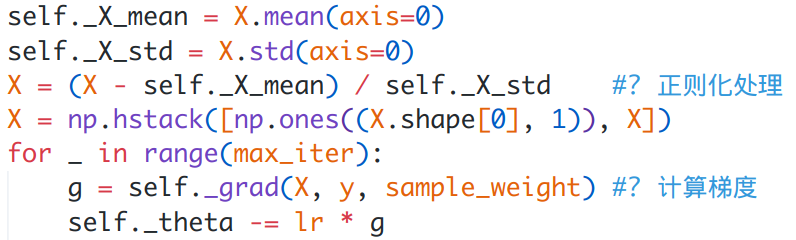
\includegraphics[scale = 0.35, frame]{images/lf.png}
    \end{center}
    \caption[short]{LogisticRegression::fit实现}
\end{figure}

梯度的计算实现见下图:
\begin{figure}[H]
    \begin{center}
        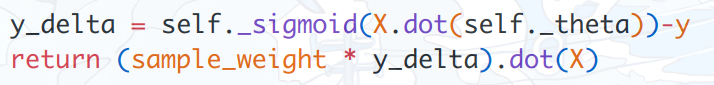
\includegraphics[scale = 0.35, frame]{images/lg.png}
    \end{center}
    \caption[short]{LogisticRegression::fit实现}
\end{figure}
            
\subsubsection{$LogisticRegression::predict(\mathbf{x})$接口实现} \label{l:p}

根据给定的$theta$、$mean$以及$std$将$\mathbf{x}$划分正负类别。

具体而言,本实验根据给定的模型参数$theta$、$mean$以及$std$计算出$\hat{y} \in (0, 1)$(逻辑回归的预测值)。接着将样本中预测值小于0.5的部分划分成负类,将样本中预测值大于等于0.5的部分划分成正类。

伪代码见算法\ref{alg:5}

\begin{algorithm}[H]
    \label{alg:5}
    \SetAlgoLined
    \caption{DecisionTreeStump:predict}
    \KwIn{数据集的特征部分$\mathbf{X}_{m \times n}$}

    $\mathbf{x}_i \leftarrow {(\mathbf{x}_i-mean) \large/ std}$ for $i \in [m]$ \tcp*[R]{正则化处理}

    $\hat{y} \leftarrow sigmoid(\theta \mathbf{X})$

    \For{$i \leftarrow 1 $ \KwTo $m$}
    {
        \eIf{$\hat{y}_i < 0.5$}
        {
            $\hat{y}_i \leftarrow -1$
        }{
            $\hat{y}_i \leftarrow 1$
        }
    }

    \KwOut{$\hat{\mathbf{y}}$}
\end{algorithm}

具体代码见下图:
\begin{figure}[H]
    \begin{center}
        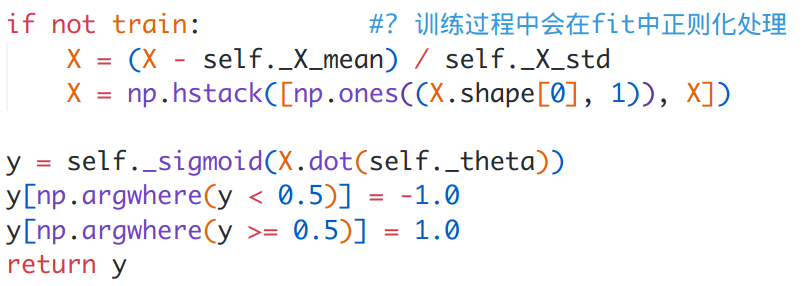
\includegraphics[scale = 0.35, frame]{images/lp.png}
    \end{center}
    \caption[short]{LogisticRegression::predict实现}
\end{figure}

\section{实验环境与平台}

\begin{itemize}
    \item OS: Manjaro Linux x86\_64
    \item Kernel: 5.15.106-1-MANJARO
    \item CPU: AMD Ryzen 7 5800H with Radeon Graphics (16) @ 3.200GHz
    \item Memory: 13832MiB
    \item Python 3.9.13 with numpy 1.21.5
\end{itemize}

\section{结果与分析}
\subsection{测试数据说明}

数据集$\mathcal{S}=\{(\mathbf{x_i},y_i)\}$,其中特征部分为$\mathbf{X}_{3679 \times 57}$,标签部分为$\mathbf{y}_{1 \times 57} \in \{0, 1\}$。

特征部分$\mathbf{X}$在各个分量上的均值见下图
\begin{figure}[H]
    \centering
    \begin{minipage}{0.48\textwidth}
        \centering
        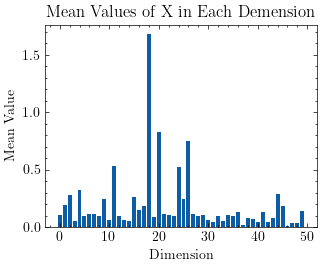
\includegraphics[scale=0.8]{images/value_of_x1.png}
        \caption{前50个维度}
    \end{minipage}
    \begin{minipage}{0.48\textwidth}
        \centering
        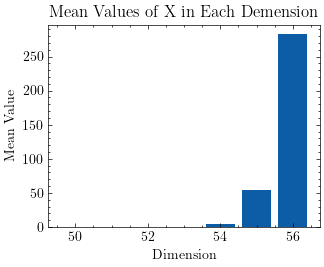
\includegraphics[scale=0.8]{images/value_of_x.png}
        \caption{50个之后的维度}
    \end{minipage}
\end{figure}

不难发现第55、56个维度上的平均值要远远大于其他维度,进行在逻辑回归算法\ref{alg:4}中进行维度正则化将有利于模型的训练和收敛。

\subsection{交折验证的方法}

在本次实验中采用了10交折验证的方法。具体而言,实验中将会首先打乱数据集,接着按照打乱后的循序依次选取10个子集作为验证集。

验证集与训练集划分的样例如下图所示:

\begin{figure}[H]
    \begin{center}
        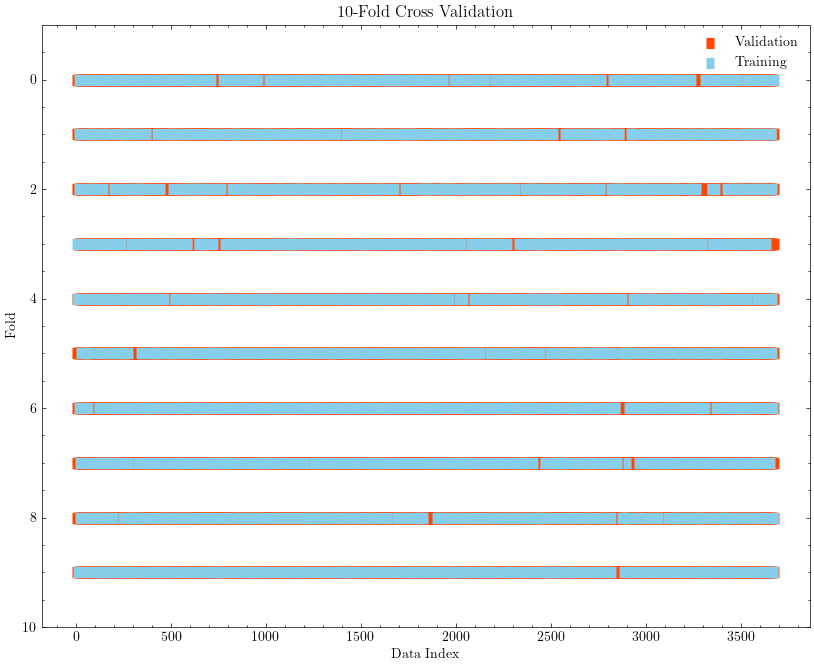
\includegraphics[scale=0.50]{images/fold.png}
    \end{center}
    \caption{Cross Validation}
\end{figure}

在本实验中,对于10-交折验证的每一个fold都分别,根据实验要求分别在基分类器数量(迭代轮数)为$\mathcal{T} \in  \{1, 5, 10, 100\}$的条件下对两种基分类器进行测试。为了便于展示结果,本实验将对$\mathcal{T} \in  \{1, 2 \dots 100\}$的测试结果用图像进行展示,对实验要求的5个迭代轮次展示具体的准确率。

\subsection{基于DecsionTreeStump分类器的Adaboost算法结果} \label{acc}

$Fold \in \{1, 2, 3, 4, 5\}$的准确率$Accuracy$随着迭代轮数$\mathcal{T}$的变化如下图所示
\begin{figure}[H]
    \centering
    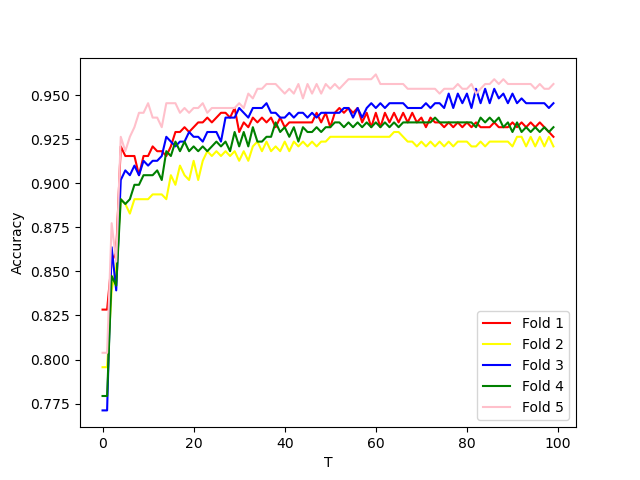
\includegraphics[scale=0.59]{images/foldacc.png}
    \caption{准确率}
\end{figure}

$Fold \in \{6, 7, 8, 9, 10\}$的准确率$Accuracy$随着迭代轮数$\mathcal{T}$的变化如下图所示
\begin{figure}[H]
    \centering
    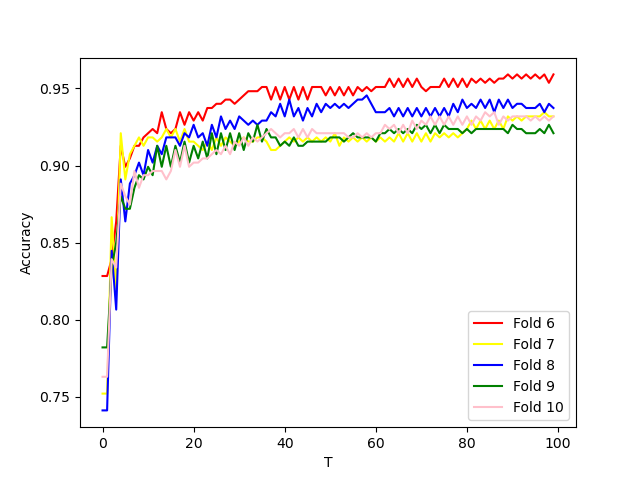
\includegraphics[scale=0.59]{images/fold1.png}
    \caption{准确率}
\end{figure}

$Fold \in \{1, 2 \dots 10\}$的准确率$Accuracy$与迭代轮数$\mathcal{T} \in \{1, 5, 10, 100\}$的关系如下表所示:

\begin{table}[H]
	\centering
	\caption{准确率}
	\begin{tabular}{|c|c|c|c|c|c|c|c|c|c|c|}
		\hline
		      & Fold1 & Fold2 & Fold3 & Fold4 & Fold5 & Fold6 & Fold7 & Fold8 & Fold9 & Fold10 \\ \hline
		T=1   & 82.83\% & 79.56\% & 77.11\% & 77.93\% & 80.38\% & 82.83\% & 75.20\% & 74.11\% & 78.20\% & 76.02\% \\ \hline
		T=5   & 92.10\% & 89.10\% & 90.19\% & 89.10\% & 92.64\% & 91.28\% & 92.10\% & 89.10\% & 88.01\% & 88.56\% \\ \hline
		T=10  & 91.55\% & 89.10\% & 91.28\% & 90.46\% & 94.01\% & 91.83\% & 91.28\% & 89.37\% & 89.10\% & 89.10\% \\ \hline
		T=100 & 92.64\% & 92.10\% & 94.55\% & 93.19\% & 95.64\% & 95.91\% & 93.19\% & 93.73\% & 92.10\% & 92.92\% \\ \hline
	\end{tabular}
\end{table}

通过上面的表格可以发现,迭代轮数(基分类器数目)$\mathcal{T}$越大,验证集的准确率也就越高。

\subsection{基于LogisitcRegression分类器的Adaboost算法结果}


$Fold \in \{1, 2, 3, 4, 5\}$的准确率$Accuracy$随着迭代轮数$\mathcal{T}$的变化如下图所示:
\begin{figure}[H]
    \centering
    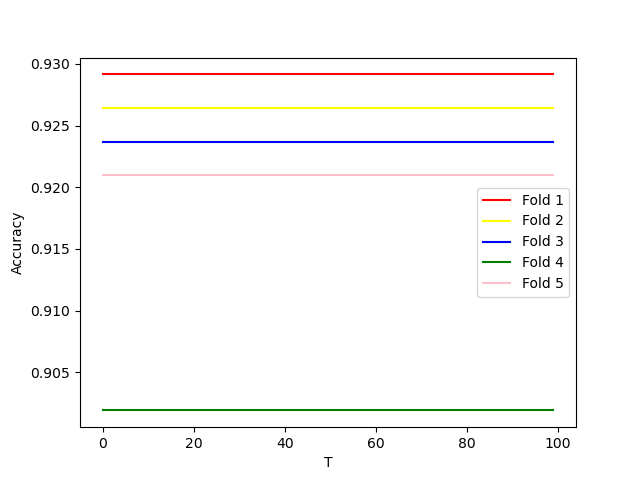
\includegraphics[scale=0.8]{images/lacc1.png}
    \caption{准确率}
\end{figure}

$Fold \in \{6, 7, 8, 9, 10\}$的准确率$Accuracy$随着迭代轮数$\mathcal{T}$的变化如下图所示:
\begin{figure}[H]
    \centering
    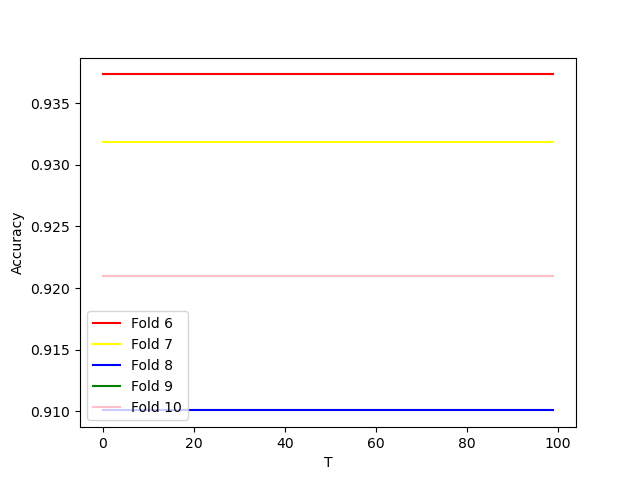
\includegraphics[scale=0.8]{images/lacc.png}
    \caption{准确率}
\end{figure}

$Fold \in \{1, 2 \dots 10\}$的准确率$Accuracy$与迭代轮数$\mathcal{T} \in \{1, 5, 10, 100\}$的关系如下表所示:

\begin{table}[htbp]
	\centering
	\caption{准确率}
	\begin{tabular}{|c|c|c|c|c|c|c|c|c|c|c|}
		\hline
		      & Fold1 & Fold2 & Fold3 & Fold4 & Fold5 & Fold6 & Fold7 & Fold8 & Fold9 & Fold10 \\ \hline
		T=1 & 92.92\% & 92.92\% & 92.37\% & 90.19\% & 92.10\% & 93.73\% & 93.19\% & 91.01\% & 92.10\% & 92.10\% \\ \hline 
        T=5 & 92.92\% & 92.92\% & 92.37\% & 90.19\% & 92.10\% & 93.73\% & 93.19\% & 91.01\% & 92.10\% & 92.10\% \\ \hline
        T=10 & 92.92\% & 92.92\% & 92.37\% & 90.19\% & 92.10\% & 93.73\% & 93.19\% & 91.01\% & 92.10\% & 92.10\% \\ \hline
        T=100 & 92.92\% & 92.92\% & 92.37\% & 90.19\% & 92.10\% & 93.73\% & 93.19\% & 91.01\% & 92.10\% & 92.10\%  \\ \hline
	\end{tabular}
\end{table}

\subsection{结果分析}\label{result}

\subsubsection{以DecisionTreeStump作为基分类器的结果}

通过观察测试结果可以发现,随着迭代轮数(分类器数目)$\mathcal{T}$的增加,对于以DecisionTreeStump算法作为分类器的Adaboost算法而言,准确率逐渐上升。

\subsubsection{以LogisticRegression作为分类算法的结果}

使用LogisticRegression作为分类算法时,准确率并不会随着$\mathcal{T}$的增加发生变化。在本实验中观察训练过程可以发现,使用LogisticRegression作为分类器的Adaboost算法并不能完整的运行完成,而会因为算法\ref{alg:1}中的第\ref{algpart:4}行错误率$err > 0.5$而退出。因此随着迭代轮数的增加,并不会有更多数目的LogisticRegression分类器被训练成型,算法每次仅会用几个固定数目的LogisticRegression分类器进行预测,因此预测的结果不会随着$\mathcal{T}$的增加发生变化。

\subsubsection{LogisticRegression作为分类器表现差的原因} \label{reason}

使用LogisticRegression作为分类算法与Adaboost算法进行结合的做法从理论角度看并不可行。这是因为LogisticRegression作为分类算法时使用的损失函数(Loss Function)如下所示:
\begin{equation} \label{form:1}
    l_i = -y_i\ln{y}_i-(\hat{y}_i-y_i)\ln{(\hat{y}_i-y_i)}
\end{equation}
\begin{equation} \label{form:2}
    Loss \leftarrow \sum_{i \in [m]}{\mathcal{D}_i \cdot l_i}
\end{equation}
其中$\hat{y}$是真实值$y$。

而Adaboost算法使用的损失函数是指数损失:
\begin{equation} \label{form:3}
    l_i = \exp{(-y_i \hat{y}_i)}
\end{equation}
在运行LogisticRegression算法时,会假设损失函数为公式\ref{form:1}以及公式\ref{form:2},并以此为基础对权重求梯度。然而Adaboost算法执行的过程中使用的损失函数为公式\ref{form:3},这导致分类器所求梯度并不是损失函数的梯度,因此分类器的权重不会被正确更新,并且错误率逐步积累,最终导致算法停止。

\section{个人体会}

\subsection{我对Adaboost算法的新认识}

\begin{enumerate}
    \item Adaboost算法的基本思想
    
            Adaboost算法的基本思想是通过训练多个弱分类器,并通过弱分类器线性拟合的方式合成一个强分类器。本实验使用的拟合方式如下:

            \begin{equation}
                H_{\mathcal{T}} = sign(\sum_{t=0}^{\mathcal{T}} \alpha h_t)
            \end{equation}
            其中$H_{\mathcal{T}}$是Adaboost算法合成的强分类器,$h_t$是迭代轮数为$t$时训练的弱分类器。

    \item Adaboost算法提供的是算法框架
    
            Adaboost算法提供的是算法框架,可以使用各种类型基分类器进行训练。但在本实验中,LogisticRegression作为基分类算法的效果并不如DecisionTreeStump,这是因为在计算的过程中LogistiRegression分类器权重的梯度并没有被正确求解,导致准确率并不会随着$\mathcal{T}$的增加而上升。具体原因见:\ref{reason}。
\end{enumerate}

\subsection{基分类器类型,超参数设置对模型性能的影响}

\begin{enumerate}

    \item 基分类器类型的影响
            
            不同的基分类器对模型的效果有着不同的影响,在本实验中以DecisionTreeStump作为基分类器要比LogisticRegression好,具体结果见:\ref{result}。
    
    \item 迭代轮数$\mathcal{T}$的影响

            随着迭代轮数$\mathcal{T}$的增加,以DecisionTreeStump算法作为基分类器的Adaboost算法模型的准确率逐渐上升。准确率达到一定程度之后就不再上升了。具体见:\ref{acc}。

\end{enumerate}

\bibliography{adaboost}

\begin{thebibliography}{99}  

    \bibitem{ref1}Robert E. Schapire, Yoav Freund, Peter Barlett, and Wee Sun Lee. Boosting the margin: A new explanation for the effectiveness of voting methods. In Proceedings of the 14th International Conference on
    Machine Learning, pages 322–330, Nashville, TN, 1997.

    \bibitem{ref2}Iba, Wayne; Langley, Pat (1992). Induction of One-Level Decision Trees.ML92: Proceedings of the Ninth International Conference on Machine Learning, Aberdeen, Scotland, 1–3 July 1992. Morgan Kaufmann. pp. 233–240.

    \bibitem{ref3}Tolles, Juliana; Meurer, William J (2016). Logistic Regression Relating Patient Characteristics to Outcomes.
    
\end{thebibliography}

\end{document}
